\chapter{Bibliography management}
\pagestyle{fancy}\lhead{\textbf \footnotesize\it{Bibliography management}}
\pagestyle{fancy}\chead{} \pagestyle{fancy}\rhead{}
\pagestyle{fancy}\lfoot{\textbf {\small\it{Univ-Mascara/Computer Science: 2024}}} 
\pagestyle{fancy}\cfoot{} \pagestyle{fancy}\rfoot{\thepage}
%%%%%%%%%%%%%%%%%%%%%%%%%%%%%%%%%%%%%%%%
\section{Introduction}\label{start5}
\section{sec1}
This part is dedicated to some basic manipulations of the text using \LaTeX. We need, generally, the following levels in a chapter of a thesis manuscript.
\section{Section}
\subsection{Sub-section}
\subsubsection{Sub-sub-section}
\paragraph{Paragraph comes without numeration}
\subparagraph{Subparagraph comes without numeration }

\section{Sizes for short sentences }
\uppercase{uppercase text};\\
\Huge{Huge Text}; \LARGE{LARGE Text}; \Large{Large Text}; \large{large Text}; \normalsize{Normal Size Text}; \small{Small Text}; \footnotesize{Footnote Size Text};\scriptsize{Script Size Text}; \tiny{Tiny text}.
\normalsize{Normal Size Text}; 
\section{Lists}
Items without numbers:
\begin{itemize}
	\item item A
	\item item B
\end{itemize}
Items with numbers:
\begin{enumerate}
	\item item 1
	\item item 2
\end{enumerate}
Hybrid mode:
\begin{itemize}
	\item 1
	\begin{enumerate}
		\item item 1a
		\item item 1b
	\end{enumerate}
	\item item 2
	\item item 3
\end{itemize}
\section{Text alignment}
From the standard \LaTeX library we can use:
\flushright{flushright to align the text to the right.  Bla Bla Bla}
\\
\flushleft{flushleft to align the text to the left. Bla Bla Bla Bla Bl}\\
More preferment commands can be  found in the package "ragged2e"

\section{Colored Text}
\color{blue}
and this  text is in blue
\color{black}
and now we return to the black color
\textcolor{red}{Text colored in red}

\section{Colored boxes}
\begin{tcolorbox}[colback=blue!5!white,colframe=blue!75!black]
	My box.
\end{tcolorbox}

\begin{tcolorbox}[colback=blue!5!white,colframe=blue!75!black,title=My title]
	My box with my title.
\end{tcolorbox}

\begin{tcolorbox}[colback=green!5!white,colframe=green!75!black]
	Upper part of my box.
	\tcblower
	Lower part of my box.
\end{tcolorbox}

\begin{tcolorbox}[colback=yellow!5!white,colframe=yellow!50!black,
	colbacktitle=yellow!75!black,title=My title]
	I can do this also with a title.
	\tcblower
	Lower part of my box.
\end{tcolorbox}

\begin{tcolorbox}[colback=yellow!10!white,colframe=red!75!black,lowerbox=invisible,
	savelowerto=\jobname_ex.tex]
	Now, we play hide and seek. Where is the lower part?
	\tcblower
	I'm invisible until you find me.
\end{tcolorbox}

\begin{tcolorbox}[colback=yellow!10!white,colframe=red!75!black,title=Here I am]
	\input{\jobname_ex.tex}
\end{tcolorbox}


\begin{tcolorbox}[enhanced,sharp corners=uphill,
	colback=blue!50!white,colframe=blue!25!black,coltext=yellow,
	fontupper=\Large\bfseries,arc=6mm,boxrule=2mm,boxsep=5mm,
	borderline={0.3mm}{0.3mm}{white}]
	Funny settings.
\end{tcolorbox}


\begin{tcolorbox}[enhanced,frame style image=blueshade.png,
	opacityback=0.75,opacitybacktitle=0.25,
	colback=blue!5!white,colframe=blue!75!black,
	title=My title]
	This box is filled with an external image.\par
	Title and interior are made partly transparent to show the image.
\end{tcolorbox}


\begin{tcolorbox}[enhanced,attach boxed title to top center={yshift=-3mm,yshifttext=-1mm},
	colback=blue!5!white,colframe=blue!75!black,colbacktitle=red!80!black,
	title=My title,fonttitle=\bfseries,
	boxed title style={size=small,colframe=red!50!black} ]
	This box uses a \textit{boxed title}. The box of the title can
	be formatted independently from the main box.
\end{tcolorbox}


\clearpage
%----------------------------------------------------------
\section{\LaTeX-Examples}

\begin{tcblisting}{colback=red!5!white,colframe=red!75!black}
	This is a \LaTeX\ example:
	\begin{equation}
		\sum\limits_{i=1}^n i = \frac{n(n+1)}{2}.
	\end{equation}
\end{tcblisting}


\begin{tcblisting}{colback=red!5!white,colframe=red!75!black,listing side text,
		title=Side by side,fonttitle=\bfseries}
	This is a \LaTeX\ example:
	\begin{equation}
		\sum\limits_{i=1}^n i = \frac{n(n+1)}{2}.
	\end{equation}
\end{tcblisting}


%----------------------------------------------------------
\section{Theorems}

\newtcbtheorem[auto counter,number within=section]{theo}%
{Theorem}{fonttitle=\bfseries\upshape, fontupper=\slshape,
	arc=0mm, colback=blue!5!white,colframe=blue!75!black}{theorem}

\begin{theo}{Summation of Numbers}{summation}
	For all natural number $n$ it holds:
	\begin{equation}
		\tcbhighmath{\sum\limits_{i=1}^n i = \frac{n(n+1)}{2}.}
	\end{equation}
\end{theo}

We have given Theorem \ref{theorem:summation} on page \pageref{theorem:summation}.

\newtcbtheorem[use counter from=theo]{antheo}%
{Theorem}{theorem style=change,oversize,enlarge top by=1mm,enlarge bottom by=1mm,
	enhanced jigsaw,interior hidden,fuzzy halo=1mm with green,
	fonttitle=\bfseries\upshape,fontupper=\slshape,
	colframe=green!75!black,coltitle=green!50!blue!75!black}{antheorem}

\begin{antheo}{Summation of Numbers}{summation}
	For all natural number $n$ it holds:
	\begin{equation}
		\tcbhighmath{\sum\limits_{i=1}^n i = \frac{n(n+1)}{2}.}
	\end{equation}
\end{antheo}

%----------------------------------------------------------
\section{Watermarks}

\begin{tcolorbox}[enhanced,watermark graphics=Figures/Logo_uzad.png,
	watermark opacity=0.3,watermark zoom=0.9,
	colback=green!5!white,colframe=green!75!black,
	fonttitle=\bfseries, title=Box with a watermark picture]
	Here, you see my nice box with a picture as a watermark.
	This picture is automatically resized to fit the dimensions
	of my box. Instead of a picure, some text could be used or
	arbitrary graphical code. See the documentation for more options.
\end{tcolorbox}

%----------------------------------------------------------
\section{Boxes in boxes}
\begin{tcolorbox}[colback=yellow!10!white,colframe=yellow!50!black,
	every box/.style={fonttitle=\bfseries},title=Box]
	\begin{tcolorbox}[enhanced,colback=red!10!white,colframe=red!50!black,
		colbacktitle=red!85!black,
		title=Box inside box,drop fuzzy shadow]
		\begin{tcolorbox}[beamer,colframe=blue!50!black,title=Box inside box inside box]
			And now for something completely different: Boxes!\par\medskip
			\newtcbox{\mybox}[1][]{nobeforeafter,tcbox raise base,colframe=green!50!black,colback=green!10!white,
				sharp corners,top=1pt,bottom=1pt,before upper=\strut,#1}
			\mybox[rounded corners=west]{This} \mybox{is} \mybox{another} \mybox[rounded corners=east]{box.}
		\end{tcolorbox}
	\end{tcolorbox}
\end{tcolorbox}



%----------------------------------------------------------
\section{Breakable Boxes}
\begin{tcolorbox}[enhanced jigsaw,breakable,pad at break*=1mm,
	colback=blue!5!white,colframe=blue!75!black,title=Breakable box,
	watermark color=white,watermark text=\Roman{tcbbreakpart}]
	\lipsum[1-12]
\end{tcolorbox}

%----------------------------------------------------------
\clearpage
\section{Fit Boxes}

\begin{tcolorbox}[enhanced,fit to height=10cm,
	colback=green!25!black!10!white,colframe=green!75!black,title=Fit box (10cm),
	drop fuzzy shadow,watermark color=white,watermark text=Fit]
	\lipsum[1-4]
\end{tcolorbox}

\begin{tcolorbox}[enhanced,fit to height=5cm,
	colback=green!25!black!10!white,colframe=green!75!black,title=Fit box (5cm),
	drop fuzzy shadow,watermark color=white,watermark text=Fit]
	\lipsum[1-4]
\end{tcolorbox}

\section{Verbatim environment}
This environment is dedicated to write codes.
\begin{Verbatim}[numbers=left, xleftmargin=5mm]
	\documentclass[11pt,a4paper,oneside]{report}
	\begin{document}
		\title{Practical Typesetting}
		\author{Peter Flynn\\Silmaril Consultants}
		\date{December 2004}
		\maketitle
	\end{document}
\end{Verbatim}

\section{sec2}
This chapter presents the basic elements for mathematics formula under \LaTeX.
\section{Inline math}
The first is $ x^n + y^n = z^n$ or (xn + yn = zn) for inline expression. \\
The second one, in separate line, is: $$ x^n + y^n = z^n$$
The third one is: \[x^n + y^n = z^n \] 
\section{Environment "math" }
\begin{math}
	x^n + y^n = z^n
\end{math}
\section{Environment "displaymath"}
\begin{displaymath}
	x^2+y^2=z^2
\end{displaymath}
\section{Environment "equation" }
Numbered equation
\begin{equation}
	x^2+y^2=z^2
	\label{eq: eqa}
\end{equation}
You can cite in the text the equation using "ref" like "Equation \ref{eq: eqa}" without () or using "eqref" "Equation \eqref{eq: eqa}" with ().\\
Non-numbered equation:
\begin{equation*}
	x^2+y^2=z^2
\end{equation*}
\section{Environment "eqnarray" }
Different styles under "eqnarray" environment:
\begin{eqnarray*}
	f(x) = \sum_{i=0}^{n} \frac{a_i}{1+x} \\
	\textstyle f(x) = \sum_{i=0}^{n} \frac{a_i}{1+x} \\
	\scriptstyle f(x) = \sum_{i=0}^{n} \frac{a_i}{1+x} \\
	\scriptscriptstyle f(x) = \sum_{i=0}^{n} \frac{a_i}{1+x}
\end{eqnarray*}
Or more sophisticated:
\[
a_0+{1\over\displaystyle a_1+
	{1\over\displaystyle a_2+
		{1 \over\displaystyle a_3 + 
			{1 \over\displaystyle a_4}}}}
\]
\section{Environment "cases"} 
$$
X(m,n)=
\begin{cases}
	x(n) & \text{if} \quad m=n \\
	x(n-1) & \text{if} \quad m>n\\
	x(n-1) & \text{if} \quad m<n.
\end{cases}
$$

\section{Environment "multline"} 
\begin{multline}
	Q(\lambda,\hat{\lambda}) = -\frac{1}{2} P(O \mid \lambda ) \sum_s \sum_m \sum_t \gamma_m^{(s)} (t) \biggl( n \log(2 \pi ) \\
	+ \log \left| C_m^{(s)} \right| + \left( \mathbf{o}_t - \hat{\mu}_m^{(s)} \right) ^T C_m^{(s)-1} \left(\mathbf{o}_t - \hat{\mu}_m^{(s)}\right) \biggr)
\end{multline}

\section{Environment "align"}
\begin{align}
	Q(\lambda,\hat{\lambda})
	= -\frac{1}{2} P(O \mid \lambda )
	\sum_s \sum_m \sum_t \gamma_m^{(s)} (t)
	\Biggl( n\log(2\pi)
	\mspace{150mu}
	\notag\\
	+ \log \left| C_m^{(s)} \right|
	+ \left( \mathbf{o}_t - \hat{\mu}_m^{(s)} \right)^T C_m^{(s)-1}
	\left(\mathbf{o}_t - \hat{\mu}_m^{(s)}\right)
	\Biggr)
\end{align}
\section{Environment "split"}
\begin{equation}
	\begin{split}
		\vec{A} \cdot \vec{B} & = (A_x \hat{x} + A_y \hat{y}+ A_z\hat{z}) \cdot (B_x \hat{x} + B_y \hat{y}+ B_z\hat{z}) \\
		& = A_xB_x(\hat{x} \cdot \hat{x}) + A_yB_y(\hat{y} \cdot \hat{y}) + A_zB_z (\hat{z} \cdot \hat{z}) \\
		&= A_xB_x + A_yB_y+A_zB_z
	\end{split}
\end{equation}
\section{Environment "alignat"}
\begin{alignat}{1}
	\frac{d\tilde{x}}{dt} &= -(\tilde{x}+x_0)\{\tilde{x}^2 + (2x_0-2)\tilde{x} + (x_0^2-2x_0-\mu_0-\tilde{\mu})\} \nonumber \\      
	\frac{d\tilde{x}}{dt} &= -\{\tilde{x}^3 + (3x_0-2)\tilde{x}^2 + (3x_0^2-4x_0-\mu_0-\tilde{\mu})\tilde{x} \\
	&{\hspace{12pt}} +(x_0^3 -2x_0^2 -x_0\mu_0 -x_0\tilde{\mu})\} \nonumber
\end{alignat} 
\section{Environment "gather"}
\begin{gather*} 
	2x - 5y =  8 \\ 
	3x^2 + 9y =  3a + c
\end{gather*}
There is also the environment "dmath" from the package "breqn".\\
If something is missing, do not hesitate to contact us at \href{mailto:guesmika@yahoo.fr}{guesmika@yahoo.fr} or read the document from the beginning section \ref{start2}. You can also read from the overleaf site \url{www.overleaf.com}.\\
The Comprehensive LaTeX Symbol List is available at this address:\\
\url{https://www.overleaf.com/articles/the-comprehensive-latex-symbol-list/czzxggzcyyqj}

\section{sec3}
We show in this chapter how to use LaTeX to create and customize tables.
\section{Environment "tabular"}
with the environment "tabular" we can create our first table:
\begin{tabular}{ c c c }
	1 & 2 & 3 \\ 
	4 & 5 & 6 \\  
	7 & 8 & 9    
\end{tabular}
\\We can center it using "center"
\begin{center}
	\begin{tabular}{ c c c }
		1 & 2 & 3 \\ 
		4 & 5 & 6 \\  
		7 & 8 & 9    
	\end{tabular}
\end{center}
For horizontal lines "hline" and vertical lines "|"
\begin{center}
	\begin{tabular}{ |c|c|c| } 
		\hline
		& A & B \\
		\hline \hline
		1 & A1 & B1 \\ 
		\hline
		2 & A2 & B2 \\ 
		\hline
	\end{tabular}
\end{center}
\section{Environment "table}
We use it to add "caption" and "label" to the tabular :
\begin{table}[]
	\centering
	\begin{tabular}{ |c|c|c| } 
		\hline
		& A & B \\
		\hline \hline
		1 & A1 & B1 \\ 
		\hline
		2 & A2 & B2 \\ 
		\hline
	\end{tabular}
	\caption{Table's caption}
	\label{tab:table0}
\end{table}
we can cite the table \ref{tab:table0} in the text.
\section{Merging cells}
\subsection{Merging columns}
\begin{tabular}{ |l|l|l|l|  }
	\hline
	\multicolumn{4}{|c|}{Merged 4 columns} \\
	\hline
	XXX & 1 & 2 & 3\\
	\hline
	A   & A1    &A2& A3\\ \hline
	B&   B1  & B2   &B3\\ \hline
	C &C1 & \multicolumn{2}{|c|}{Merged 2 columns}\\
	\hline
\end{tabular}

\subsection{Merging lines} 
To merge lines you need to add the "multirow" package to your document preamble.
\begin{center}
	\begin{tabular}{ |c|c|c|c| } 
		\hline
		col1 & col2 & col3 \\
		\hline
		\multirow{3}{4em}{Merged lines} & cell 2 & cell 3 \\ 
		& cell 5 & cell 6 \\ 
		& cell 8 & cell 9 \\ 
		\hline
	\end{tabular}
\end{center}

\section{Positioning tables}
As a floating element you can specify the table position using one commutator of the following: (h=here, t=top, b=bottom, p=special page, !=Override internal \LaTeX parameters, H=Place the table at this precise location=!h)
\newpage

\subsubsection{Examples}
In this page two tables at the top and the bottom of the page.
\begin{table}[t]
	\centering
	\begin{tabular}{ |c|c|c| } 
		\hline
		& A & B \\
		\hline \hline
		1 & A1 & B1 \\ 
		\hline
		2 & A2 & B2 \\ 
		\hline
	\end{tabular}
	\caption{Table on top }
	\label{tab:table0}
\end{table}

\begin{table}[h]
	\centering
	\begin{tabular}{ |c|c|c| } 
		\hline
		& A & B \\
		\hline \hline
		1 & A1 & B1 \\ 
		\hline
		2 & A2 & B2 \\ 
		\hline
	\end{tabular}
	\caption{Table on here }
	\label{tab:table0}
\end{table}

\begin{table}[b]
	\centering
	\begin{tabular}{ |c|c|c| } 
		\hline
		& A & B \\
		\hline \hline
		1 & A1 & B1 \\ 
		\hline
		2 & A2 & B2 \\ 
		\hline
	\end{tabular}
	\caption{Table on bottom }
	\label{tab:table0}
\end{table}
\newpage
\section{Columns with fixed length} 
we use the package "array" to fix the columns length. 1st column of width=5em centered (m=middle) the 2nd of length=5cm
\begin{table}[H]
	\begin{center}
		\begin{tabular}{ | m{5em} | m{5cm}| m{1cm} | } 
			\hline
			Bla Bla Bla Bla & cell2 & cell3 \\ 
			\hline
			Bla Bla Bla Bla Bla  & cell5 & cell6 \\ 
			\hline
			cell7 & cell8 & cell9 \\ 
			\hline
		\end{tabular}
	\end{center}
	\caption{Columns with fixed length}
	%\label{tab:table0}
\end{table}

We can fix also the whole table length and this last will equi-dispatched between columns. This is possible using "tabularx" package.
\begin{tabularx}{0.8\textwidth} { 
		| >{\raggedright\arraybackslash}X 
		| >{\centering\arraybackslash}X 
		| >{\raggedleft\arraybackslash}X | }
	\hline
	item 11 & item 12 & item 13 \\
	\hline
	item 21  & item 22  & item 23  \\
	\hline
\end{tabularx}
\section{List of tables}
To create a list of tables use the command "listoftables" (see result on the next page) .
\listoftables
\newpage

\section{sec4}
This chapter is dedicated to the float element: Figure. Of course you need "graphicx" package to create a figure and "float" to give it a position.  
(h=here, t=top, b=bottom, p=special page, !=Override internal \LaTeX parameters, H=Place the figure at this precise location=!h)
\section{First figure}
\begin{figure}[H]
	\centering
	\includegraphics[scale=1.5]{Figures/Logo_uzad.png}
	\caption{Djelfa university logo}
\end{figure}
\subsection{Subfigures}
You need the "subcaption" package
\begin{figure}[H]
	\begin{subfigure}{.3\textwidth}
		\centering
		\includegraphics[width=0.75\textwidth]{Figures/fig3.2.PNG}
		\caption{Sub Fig 1}
	\end{subfigure}
	%%%%%%%%%%%%%%
	\begin{subfigure}{.3\textwidth}
		\centering
		\includegraphics[width=0.75\textwidth]{Figures/Logo_uzad.png}
		\caption{Sub Fig 2}
	\end{subfigure}
	%%%%%%%%%%%%%%
	\begin{subfigure}{.3\textwidth}
		\centering
		\includegraphics[width=0.75\textwidth]{Figures/fig3.3.PNG}
		\caption{Sub Fig 3}
	\end{subfigure}
	\caption{Set of Sub Figures}
\end{figure}
You can create also a matrix of sub figures:
\begin{figure}[H]
	\centering
	\begin{tabular}{cc}
		\begin{subfigure}{.3\textwidth}
			\centering
			\includegraphics[width=0.75\textwidth]{Figures/Logo_uzad.PNG}
			\caption{Sub Fig 1}
		\end{subfigure} 
		&  
		\begin{subfigure}{.3\textwidth}
			\centering
			\includegraphics[width=0.75\textwidth]{Figures/Logo_uzad.PNG}
			\caption{Sub Fig 2}
		\end{subfigure} 
		\\
		\begin{subfigure}{.3\textwidth}
			\centering
			\includegraphics[width=0.75\textwidth]{Figures/Logo_uzad.PNG}
			\caption{Sub Fig 3}
		\end{subfigure}
		& 
		\begin{subfigure}{.3\textwidth}
			\centering
			\includegraphics[width=0.75\textwidth]{Figures/Logo_uzad.PNG}
			\caption{Sub Fig 4}
		\end{subfigure}
	\end{tabular}
	\caption{Matrix of Sub Figures}
	\label{fig: mat_fig}	
\end{figure}

\section{List of figures}
You can add to your document the list of figures using the command "listoffigures". See result on the next page.
\listoffigures
\section{Dimensions of figure}
To specify the dimension of a figure, you need some commands and to know about units such as:\\
\begin{table}[H]
	\centering
	\begin{tabular}{|c|c|c|}
		\hline
		Command & Use for & Expl of use \\ \hline
		\verb=\columnsep= & distance between columns & \the \columnsep \\ \hline
		\verb=\columnwidth= &	width of the column  & \the \columnwidth \\ \hline
		\verb=\linewidth= &	width of the line in the current environment  & \the \linewidth \\\hline
		\verb=\paperwidth= & width of the page  & \the \paperwidth \\\hline
		\verb=\paperheight= & height of the page  & \the \paperheight \\\hline
		\verb=\textwidth= & width of the text  & \the \textwidth \\\hline
		\verb=\textheight= & height of the text  & \the \textheight \\\hline
		\verb=\unitlength= & units of length in the picture environment  & \the \unitlength \\\hline
	\end{tabular} 
	\caption{Dimensions}
	\label{tab:Dim_tab}
\end{table}
To specify the unit you can use one of the following:
\begin{table}[H]
	\centering
	\begin{tabular}{|c|c|}
		\hline
		Unite & meaning  \\ \hline
		pt & point  \\ \hline 
		mm & millimetre  \\ \hline 
		cm & centimetre  \\ \hline 
		in & inch  \\ \hline 
		ex & height of an x in the current font \\ \hline
		em & width of an m in the current font  \\ \hline 
	\end{tabular}
	\caption{Units}
	\label{tab:Uni_tab}
\end{table}
\section{Plots}
To plot in \LaTeX you need packages "Tikz" and "pgfplots". 
\subsection{2D Plots}
We start by an example of 2D illustration of the functions $y_1=1-x^2$ "blue colored" and $y_2=x^2$ "red colored".
\begin{figure}[H]
	\centering
	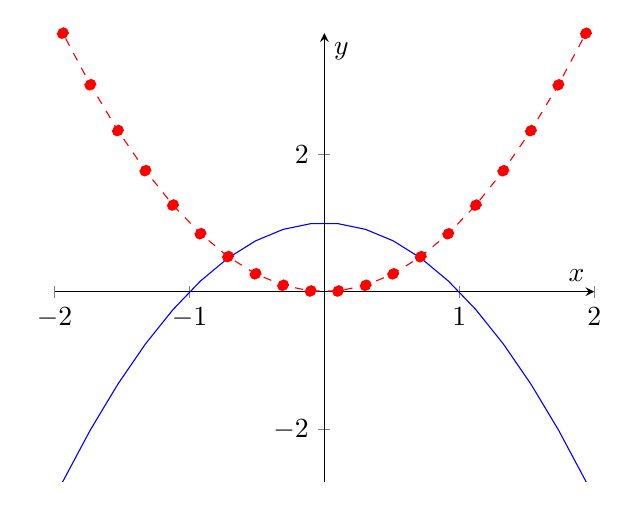
\begin{tikzpicture}
		\begin{axis}[xmin=-2, xmax=2, axis lines=middle, grid style={line width=.1pt}, xlabel={$x$}, ylabel={$y$}]
			\addplot[color=red,dashed, mark=*, samples=50]{x^2};
			\addplot[color=blue, samples=50]{1-x^2};
		\end{axis}
	\end{tikzpicture}
	\caption{2D plot of $y_1=1-x^2$ and $y_2=x^2$  }
	\label{fig:Plot_3d}
\end{figure}

\subsection{3D plots}
Here is an example of 3D illustration of the function $z=cos(y) + sin(x)$.
\begin{figure}[H]
	\centering
	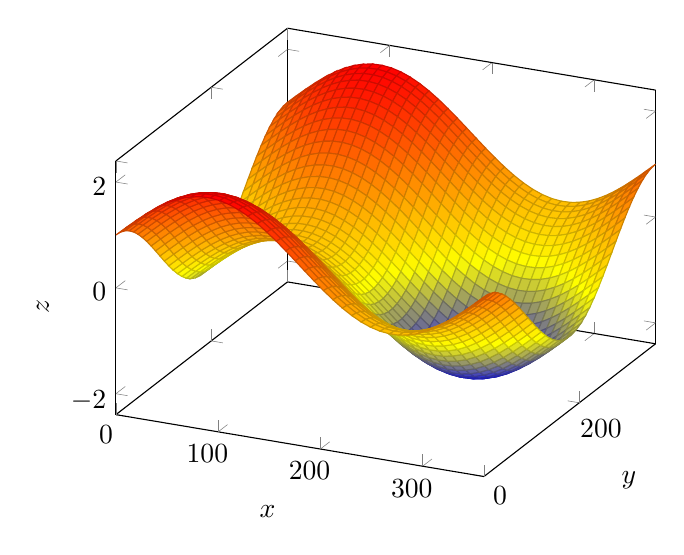
\begin{tikzpicture}
		\begin{axis}[xlabel={$x$}, ylabel={$y$}, zlabel={$z$}]
			\addplot3[surf,domain=0:360,
			samples=40] {cos(y) + sin(x)};
		\end{axis}
	\end{tikzpicture}
	\caption{3D plot of the function $Z=cos(y) + sin(x)$}
	\label{fig:Plot_3d}
\end{figure}

\section{sec5}
This part is dedicated to the main ways to insert a bibliography in your document.
\section{First way}
This is probably the simplest way. We have an external file "Biblio.bib" that contains the bibliography items.
For example, this is the first item of our bibliography \cite{01} from the whole bibliography that we can print it (for this action you need the "biblatex" package) as follows (to see the result on the next page activate \verb=\printbibliography= in the next line):
%\printbibliography

\section{Second way}
This way allows you to be free to define the bibliography style; however it is preferred for short reports with few bibliography items. In this way the same file contains the main document
and the bibliography items under the environement "thebibliography"
We can cite the second reference as: \cite{ref2}
\begin{thebibliography}{9}% we specify a max of 9 items, you can use till 99 items
	\bibitem{ref1}
	K. GUESMI (2000), Contribution to the control of DC motor, \textit{Djelfa University Press}.
	\bibitem{ref2}
	A. REBAI (2021) \emph{Asymptotic Stabilization of Fractional Order Fuzzy Time-Varying Delay Systems},2021 Global Congress on Electrical Engineering.
\end{thebibliography}
\section{Third way}
This way is the most professional and used by scientists. It consists of an external file "Biblio.bib" and we insert before the \verb=\end{document}= the following lines:
\begin{verbatim}
\nocite{*} % to insert all bibliography items cited in the text or not
\bibliographystyle{unsrt} % Order of items is by appearance 
\bibliography{Biblio} % indicate the file containing bibliography items
\end{verbatim} 
now you return to the document to cite bibliography items like the first one \cite{01}, the second one \cite{02} or the fifth one \cite{05}. That's all.\\ 
Unlike the previous way, here you will find the bibliography list at the end of your document.
\section{Conclusion}
If anything is missing, do not hesitate to contact us at \href{mailto:guesmika@yahoo.fr}{guesmika@yahoo.fr} or re-read the document from the beginning section \ref{start5}. You can also read the documentation from the web site \url{www.overleaf.com}.\\
More materials are available at:\\
\url{https://www.overleaf.com/learn/latex/Bibliography_management_with_bibtex}





